\documentclass[conference]{IEEEtran}

\usepackage{iftex}
\ifPDFTeX
  \usepackage[utf8]{inputenc}
  \usepackage[T1]{fontenc}
\fi
\usepackage[spanish,es-tabla,es-noshorthands]{babel}
\addto\captionsspanish{\renewcommand{\IEEEkeywordsname}{Palabras clave}}
\usepackage{amsmath,amssymb}
\usepackage{graphicx}
\usepackage{booktabs}
\usepackage{array}
\usepackage{cite}
\usepackage[hidelinks]{hyperref}

\graphicspath{{figuras/}}

\begin{document}

\title{Control Digital 2-DOF y Filtrado Pasabajas en Tiempo Real para un Bic\'{o}ptero sobre Riel Vertical}

% EDITAR AUTORES AQUI
\author{
  \IEEEauthorblockN{Leonardo Monter Rizo\IEEEauthorrefmark{1} y [Nombre del Colaborador]\IEEEauthorrefmark{1}}
  \IEEEauthorblockA{\IEEEauthorrefmark{1}Ingenier\'{i}a Mecatr\'{o}nica / Control y Procesamiento Digital de Se\~{n}ales\\
  Universidad An\'{a}huac, Semestre 8 (Ago--Dic 2026)\\
  Repositorio: \texttt{bicopter-rail-2dof} (rama \texttt{reporte-final-dsp-control})}
}

\maketitle

\begin{abstract}
Este reporte presenta el dise\~{n}o, la identificaci\'{o}n experimental y la validaci\'{o}n en vuelo real de un sistema de control digital y procesamiento digital de se\~{n}ales (DSP) para un bic\'{o}ptero de dos grados de libertad (altura e inclinaci\'{o}n) montado sobre un riel vertical de $20\text{ cm}$. En pruebas din\'{a}micas se encontr\'{o} que el sensor \'{o}ptico VL53L0X introduce saltos impulsivos de hasta $\pm 10\text{ mm}$ y concentra $59.1\%$ de su ruido por encima de $2\text{ Hz}$. Para resolverlo sin introducir retardos desestabilizadores, se implement\'{o} un banco de cinco filtros digitales intercambiables en tiempo de ejecuci\'{o}n (\texttt{FILTER,0..4}) que permiti\'{o} evaluar todos los candidatos en vuelo senoidal real ($12\text{ s}$, $0.35\text{ Hz}$) sin reiniciar el ESP32 ni disparar el \textit{failsafe} de los ESCs. El filtro ganador, \texttt{Median3 + Butterworth} de segundo orden ($f_c = 1.5\text{ Hz}$), redujo el ruido pico-a-pico en $38.3\%$ frente al filtro EMA base ($7.37\text{ mm}$ frente a $11.95\text{ mm}$). Finalmente, se ajust\'{o} la planta experimental $G(s)$ y $G(z)$ ($T_s = 0.05\text{ s}$, $R^2 = 0.9250$) y se formul\'{o} el modelo linealizado en espacio de estados 2-DOF, confirmando controlabilidad y observabilidad completas (rango $4/4$).
\end{abstract}

\begin{IEEEkeywords}
Bic\'{o}ptero 2-DOF, control digital PID, filtro Butterworth IIR, transformada $Z$, espacio de estados, ESP32, VL53L0X, BNO055.
\end{IEEEkeywords}

\section{Introducci\'{o}n y Evoluci\'{o}n del Prototipo}
Un bic\'{o}ptero restringido a un riel vertical de $20\text{ cm}$ ($200\text{ mm}$) constituye un banco ideal para conectar la teor\'{i}a de control digital y el procesamiento de se\~{n}ales con problemas f\'{i}sicos reales: fricci\'{o}n de corredera, vibraci\'{o}n mec\'{a}nica de h\'{e}lices, latencia de sensores I\textsuperscript{2}C y saturaci\'{o}n de actuadores. Aunque en papel los ejes de altura ($z$) e inclinaci\'{o}n ($\theta$) pueden desacoplarse mediante una mezcla suma/diferencia de empuje, en el banco f\'{i}sico el ruido impulsivo del tel\'{e}metro l\'{a}ser VL53L0X se propaga al t\'{e}rmino derivativo del PID y provoca oscilaciones innecesarias en los motores.

El desarrollo del sistema no fue lineal; evolucion\'{o} a trav\'{e}s de decisiones pr\'{a}cticas documentadas en los registros de laboratorio (\texttt{worklog1..29} en \texttt{v0.1} y \texttt{worklog1..8} en \texttt{v2.0}), resumidas en la Fig.~\ref{fig:evolucion}:
\begin{itemize}
  \item \textbf{Base segura y hardware (\texttt{v0.1}):} se estableci\'{o} arranque seguro a $1000\text{ }\mu\text{s}$ (motores desarmados), PCB monocapa auditada a $300\text{ DPI}$ y consola impresa en 3D.
  \item \textbf{Gimbal lock $\rightarrow$ cuaterniones:} durante pruebas del BNO055 cerca de $90^\circ$ se detect\'{o} singularidad en \'{a}ngulos de Euler, por lo que se valid\'{o} la orientaci\'{o}n con cuaterniones y operaci\'{o}n en modo \texttt{IMUPLUS} (6-DOF sin magnet\'{o}metro para evitar interferencia electromagn\'{e}tica de los motores).
  \item \textbf{Consola V8/V9 y panel de 4 rutinas:} se integr\'{o} un panel Web Serial con modo manual, autom\'{a}tico, control por gestos offline (MediaPipe) y cuatro botones en un clic que reescalan autom\'{a}ticamente las ganancias al tope real capturado del riel ($20\text{ cm}$).
  \item \textbf{Pivote pragm\'{a}tico de Kalman a banco pasabajas:} un filtro de Kalman de tres estados result\'{o} innecesariamente fr\'{a}gil ante saltos no gaussianos del VL53L0X a $\sim 10.6\text{ Hz}$. Sustituirlo por una etapa no lineal de mediana de 3 muestras (\texttt{Median3}) seguida de un filtro pasabajas lineal simplific\'{o} la sintonizaci\'{o}n y dio mejores resultados en vuelo.
  \item \textbf{Hallazgo de \textit{failsafe} en ESCs:} al reflashear el ESP32 entre corridas, los pines PWM quedaban sin se\~{n}al por $\sim 15\text{ s}$ y los ESCs entraban en protecci\'{o}n. Se resolvi\'{o} a\~{n}adiendo cambio de filtro en vivo (\texttt{FILTER,0..4}) y apertura serial sin reinicio (\texttt{DTR/RTS = False}).
\end{itemize}

\begin{figure*}[t]
  \centering
  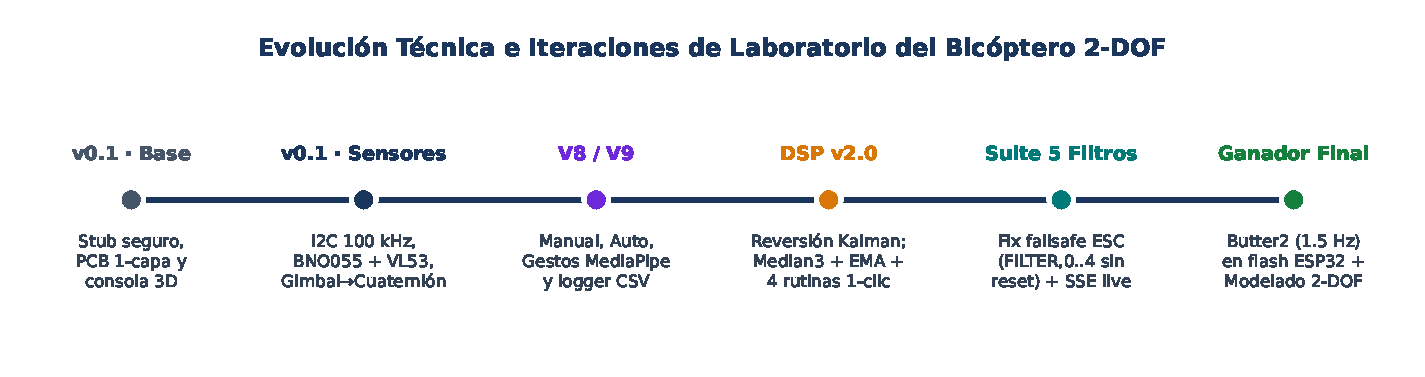
\includegraphics[width=0.96\textwidth]{fig6_evolucion_proyecto.pdf}
  \caption{L\'{i}nea de tiempo de las iteraciones de hardware, firmware y DSP que llevaron a la versi\'{o}n final en \texttt{version-prueba-v9}.}
  \label{fig:evolucion}
\end{figure*}

\section{Arquitectura del Sistema Retroalimentado}
La plataforma se apoya en un microcontrolador ESP32 \cite{espressif_esp32} que ejecuta un lazo de control digital a $f_s = 20\text{ Hz}$ ($T_s = 0.05\text{ s}$) sobre dos perif\'{e}ricos principales conectados a un bus I\textsuperscript{2}C compartido a $100\text{ kHz}$ (\texttt{GPIO21/22}):
\begin{enumerate}
  \item \textbf{VL53L0X (\texttt{0x29}):} mide distancia vertical en modo continuo con presupuesto de $50\text{ ms}$ \cite{st_vl53l0x}. Solo se aceptan lecturas con \texttt{deviceStatus == 11} y distancia $< 8190\text{ mm}$. Al encender, el sistema exige 30 muestras consecutivas con dispersi\'{o}n $\le 10\text{ mm}$ para fijar el cero del piso (\texttt{STATE,READY}).
  \item \textbf{BNO055 (\texttt{0x28}):} opera en fusi\'{o}n \texttt{IMUPLUS} (\texttt{0x08}) leyendo aceler\'{o}metro, giroscopio, Euler y cuaterniones \cite{bosch_bno055}. Al armar, la inclinaci\'{o}n actual se captura como $0^\circ$ relativo.
  \item \textbf{Actuadores ESC (\texttt{GPIO25/26}):} se\~{n}al PWM a $50\text{ Hz}$ mediante LEDC de $16\text{ bits}$ ($1000\text{--}1990\text{ }\mu\text{s}$). Al armar, ambos motores suben en rampa a $1450\text{ }\mu\text{s}$ en $1\text{ s}$ y luego obedecen una velocidad m\'{a}xima de cambio de $200\text{ }\mu\text{s/s}$.
\end{enumerate}

La telemetr\'{i}a viaja a $115200\text{ baud}$ hacia dos clientes locales complementarios: \texttt{dashboard.html} (Web Serial en puerto \texttt{8080}) para operaci\'{o}n diaria y \texttt{dsp\_live.html} (servidor SSE en puerto \texttt{8090}) para visualizaci\'{o}n en vivo de se\~{n}al cruda, filtrada y PWM durante los experimentos. La Fig.~\ref{fig:diagrama} resume el lazo cerrado completo, incluyendo el supervisor de seguridad que corta motores inmediatamente si el latido (\texttt{HB}) supera $350\text{ ms}$ o si un sensor deja de actualizarse por m\'{a}s de $200\text{ ms}$.

\begin{figure*}[t]
  \centering
  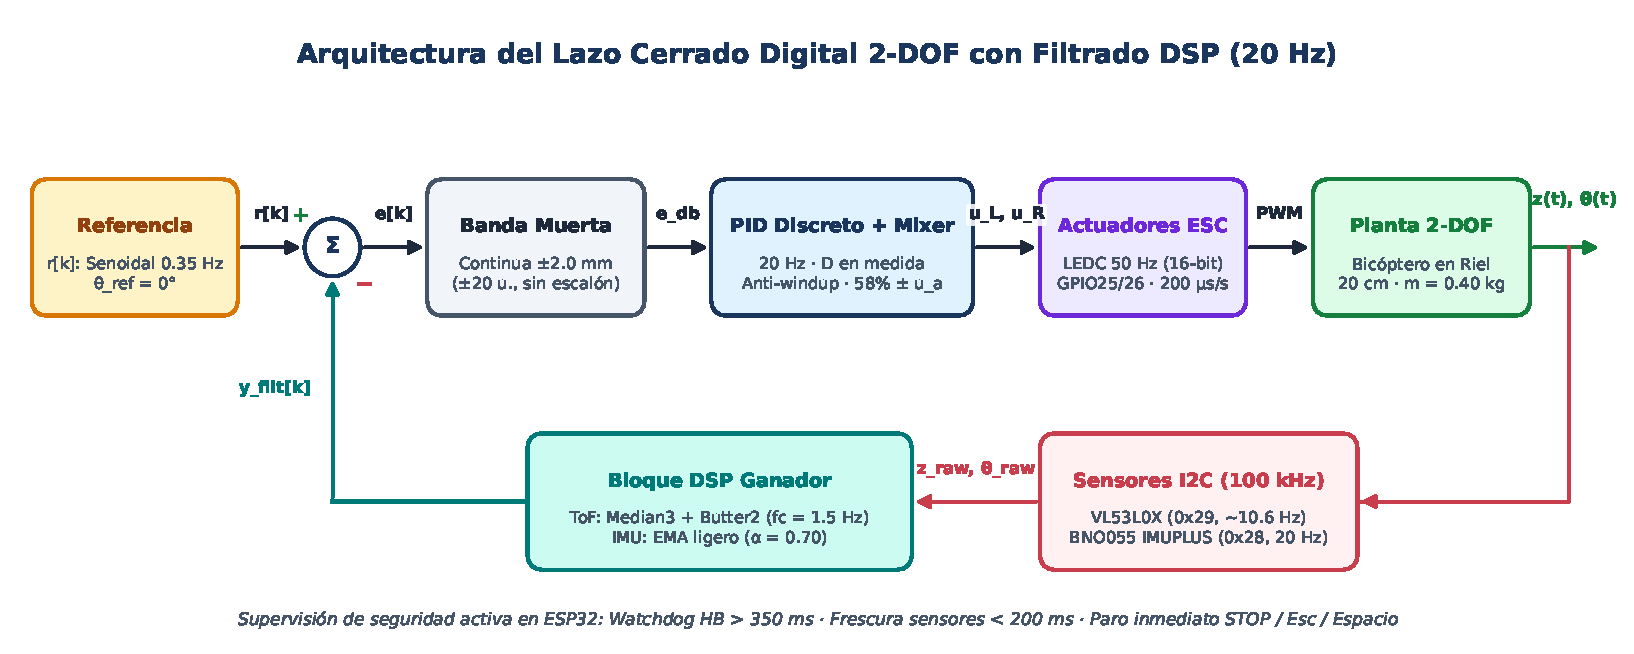
\includegraphics[width=0.98\textwidth]{fig1_diagrama_retroalimentado.pdf}
  \caption{Diagrama de bloques completo del sistema retroalimentado digital 2-DOF a $20\text{ Hz}$, incluyendo banda muerta continua, PID discreto con anti-windup, actuadores ESC y cadena DSP ganadora en la rama de realimentaci\'{o}n.}
  \label{fig:diagrama}
\end{figure*}

\section{An\'{a}lisis Espectral y Selecci\'{o}n del Filtro Digital}

\subsection{Caracterizaci\'{o}n del Ruido en Vuelo Real}
En reposo, un sensor suele parecer m\'{a}s limpio de lo que realmente es en operaci\'{o}n. Por eso se captur\'{o} primero un vuelo senoidal din\'{a}mico de $12\text{ s}$ (\texttt{dsp\_flight\_baseline.csv}) con los motores energizados. El an\'{a}lisis de frecuencias con ventana Hann \cite{vignolo_sistemas,cayetano_dsp} revel\'{o} dos fen\'{o}menos concretos (Fig.~\ref{fig:fft}):
\begin{itemize}
  \item \textbf{Tasa real asim\'{e}trica:} aunque el lazo de control e IMU corren a $21.28\text{ Hz}$, el VL53L0X entrega muestras nuevas a $10.64\text{ Hz}$.
  \item \textbf{Ruido impulsivo + alta frecuencia:} en $12\text{ s}$ se registraron $28$ saltos bruscos de $5\text{--}10\text{ mm}$ y $5$ picos $\ge 10\text{ mm}$. En el espectro PSD, el ruido din\'{a}mico reparti\'{o} $1.83\%$ en $0\text{--}1\text{ Hz}$, $39.03\%$ en $1\text{--}2\text{ Hz}$, $33.79\%$ en $2\text{--}5\text{ Hz}$ y $25.35\%$ en $5\text{--}10\text{ Hz}$ ($59.14\%$ por encima de $2\text{ Hz}$).
\end{itemize}

Como la referencia senoidal oscila a $0.35\text{ Hz}$, existe una separaci\'{o}n limpia entre el movimiento \'{u}til ($< 1\text{ Hz}$) y la mayor parte del ruido del sensor ($> 1.5\text{ Hz}$).

\begin{figure*}[t]
  \centering
  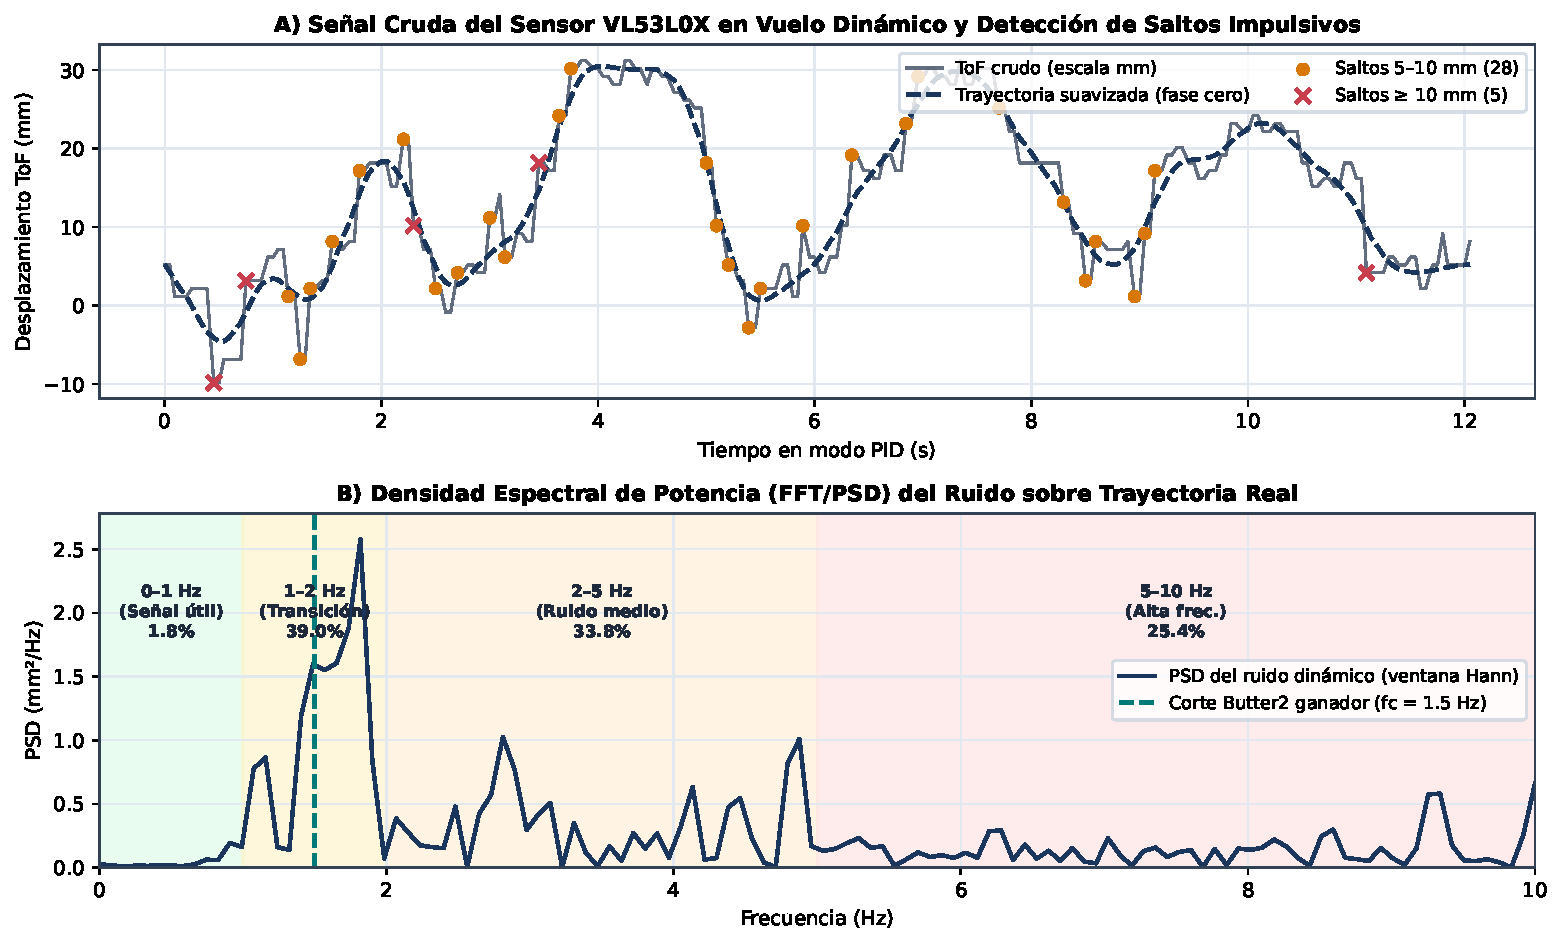
\includegraphics[width=0.88\textwidth]{fig2_espectro_fft_ruido.pdf}
  \caption{A) Se\~{n}al cruda del VL53L0X durante el vuelo din\'{a}mico con saltos impulsivos marcados. B) Densidad espectral de potencia (PSD) del residuo de ruido y ubicaci\'{o}n de la frecuencia de corte $f_c = 1.5\text{ Hz}$.}
  \label{fig:fft}
\end{figure*}

\subsection{Comparativa de los Cinco Filtros en Vuelo Real}
Un filtro lineal por s\'{i} solo convierte un pico aislado de $10\text{ mm}$ en una protuberancia alargada. Por ello, todos los candidatos comparten un pre-filtro no lineal de mediana de 3 muestras (\texttt{Median3}) que descarta picos de un solo instante sin meter retardo de fase en se\~{n}ales suaves. Sobre esa salida se probaron cinco familias pasabajas en el ESP32 \cite{vignolo_filtros,cayetano_dsp}: EMA ($\alpha = 0.30$), SMA ($N = 5$), Butterworth 2\textsuperscript{o} orden ($f_c = 1.5\text{ Hz}$), Bessel 2\textsuperscript{o} orden ($f_c = 2.0\text{ Hz}$) y Chebyshev Tipo I 2\textsuperscript{o} orden ($f_c = 1.8\text{ Hz}$, rizado $0.5\text{ dB}$ con ganancia DC normalizada a $1$).

La Tabla~\ref{tab:filtros} y la Fig.~\ref{fig:bode} muestran el desempe\~{n}o real de los cinco vuelos consecutivos ($12\text{ s}$ cada uno, todos con despegue confirmado y mismo juego de ganancias). En t\'{e}rminos f\'{i}sicos, un filtro Butterworth tiene respuesta \textit{m\'{a}ximamente plana}: deja pasar intacta la onda lenta de $0.35\text{ Hz}$ sin deformarla ni amplificarla, y aten\'{u}a con pendiente de $-40\text{ dB/d\'{e}cada}$ las vibraciones arriba de $1.5\text{ Hz}$. Por el contrario, Chebyshev y Bessel dejaron pasar la banda de $1\text{--}2\text{ Hz}$, generando sobreimpulsos hasta $1108$ y $987$ unidades (rozando el tope mec\'{a}nico).

\begin{table*}[t]
  \centering
  \caption{Resultados Experimentales de los Cinco Filtros Pasabajas en Vuelo Senoidal Real (\texttt{COM4}, $12\text{ s}$ c/u, sin Reinicio)}
  \label{tab:filtros}
  \resizebox{\textwidth}{!}{%
  \begin{tabular}{@{}lccccccccc@{}}
    \toprule
    \textbf{Filtro (con pre-filtro Median3)} & \textbf{Modo} & \textbf{Orden} & \textbf{$f_c$ (Hz)} & \textbf{Altura m\'{a}x. (u.)} & \textbf{STD (mm)} & \textbf{P2P (mm)} & \textbf{RMSE (mm)} & \textbf{PWM Jitter} & \textbf{Score} \\
    \midrule
    \textbf{Butterworth 2\textsuperscript{o} (Ganador)} & \textbf{2} & \textbf{2} & \textbf{1.50} & \textbf{878.97} & \textbf{1.692} & \textbf{7.369} & \textbf{50.20} & \textbf{0.9895} & \textbf{54.7} \\
    SMA ($N=5$) & 1 & 4 (FIR) & 1.77 & 899.67 & 1.874 & 9.307 & 49.81 & 0.9918 & 50.3 \\
    EMA ($\alpha=0.30$, base) & 0 & 1 & 1.36 & 745.78 & 1.895 & 11.945 & 44.26 & 0.9882 & 48.5 \\
    Bessel 2\textsuperscript{o} & 3 & 2 & 2.00 & 987.30 & 2.579 & 17.967 & 55.02 & 0.9876 & 29.4 \\
    Chebyshev I 2\textsuperscript{o} ($0.5\text{ dB}$) & 4 & 2 & 1.80 & 1108.00 & 3.447 & 25.306 & 57.36 & 0.9863 & 9.1 \\
    \bottomrule
  \end{tabular}}
\end{table*}

\begin{figure*}[t]
  \centering
  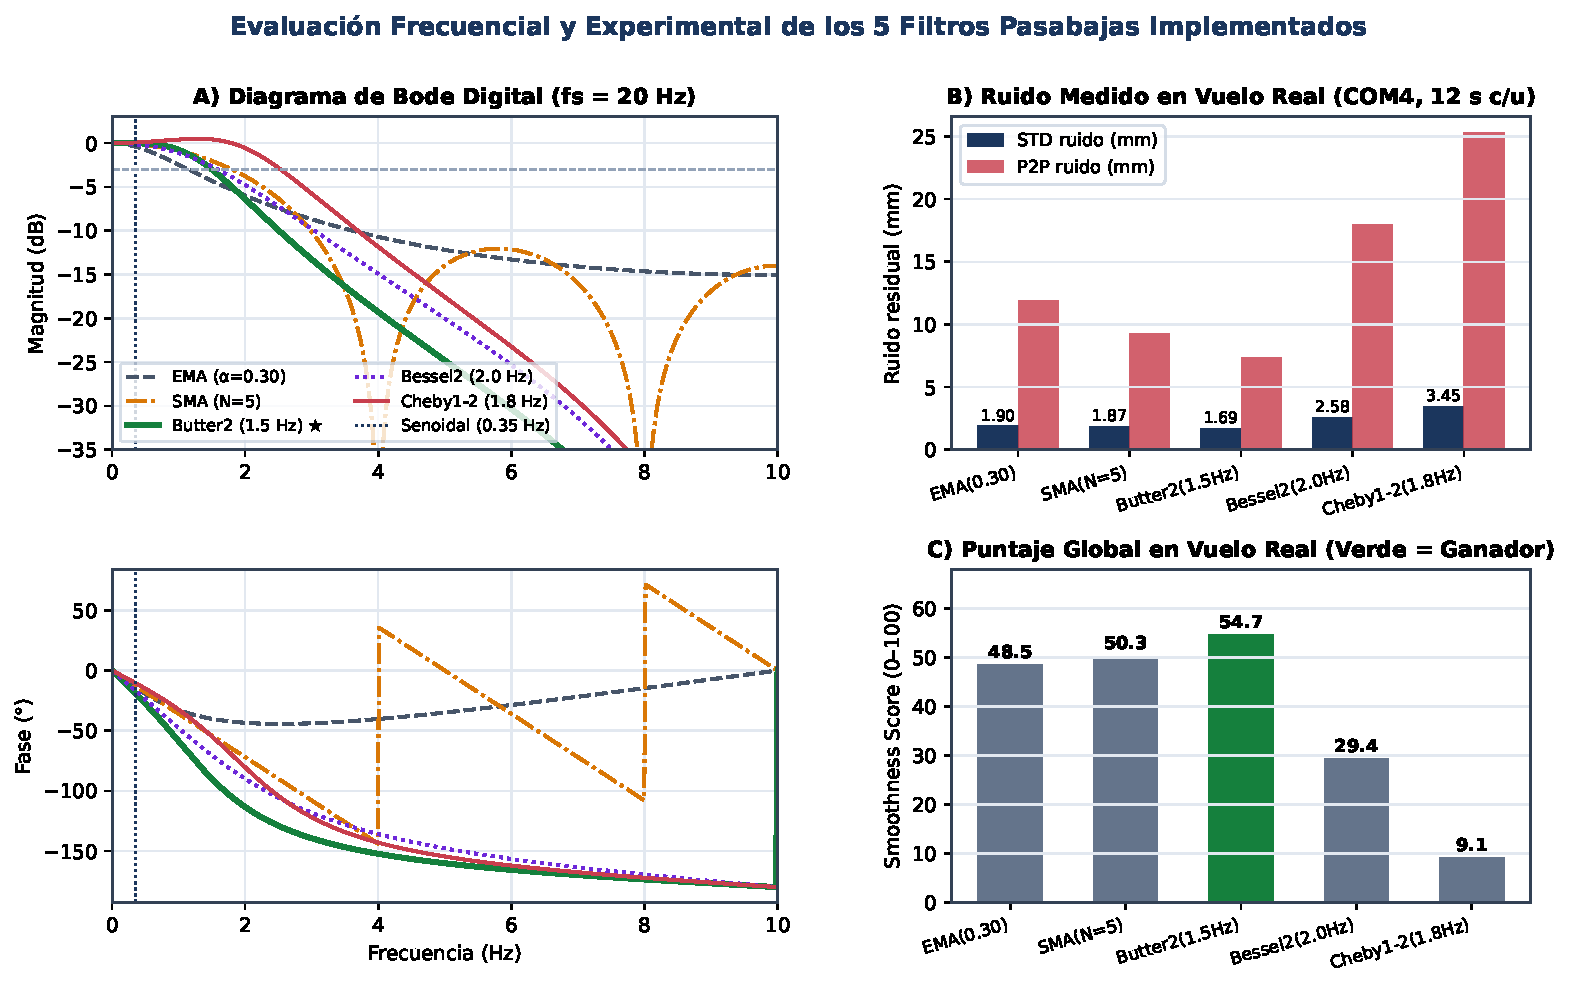
\includegraphics[width=0.96\textwidth]{fig3_comparativa_filtros.pdf}
  \caption{A) Diagrama de Bode digital a $f_s = 20\text{ Hz}$ de los cinco filtros implementados. B) Desviaci\'{o}n est\'{a}ndar y ruido pico-a-pico medidos en vuelo real. C) Puntaje global en vuelo real resaltando \texttt{Butter2 (1.5 Hz)} como ganador.}
  \label{fig:bode}
\end{figure*}

En una segunda prueba de desempate (\textit{rematch}) entre \texttt{Butter2} y \texttt{EMA}, \texttt{EMA} redujo ligeramente el ruido ($1.39\text{ mm}$ vs. $1.59\text{ mm}$) a costa de recortar la amplitud de vuelo ($639.9$ u. frente a $763.5$ u. de \texttt{Butter2} para una referencia de pico $800$ u.). Se eligi\'{o} definitivamente \texttt{Median3 + Butter2 (1.5 Hz)} en la memoria flash del ESP32 (\texttt{DSP\_FILTER\_MODE = 2}) por ofrecer mejor seguimiento sin sacrificar suavidad.

\subsection{Ecuaci\'{o}n en Diferencias del Filtro Ganador}
La transformada $Z$ traduce un filtro continuo a operaciones aritm\'{e}ticas simples que el ESP32 ejecuta en microsegundos \cite{vignolo_sistemas,vignolo_filtros}. Tras calcular la mediana $m[k] = \operatorname{med}(d[k], d[k-1], d[k-2])$ y restar el origen $x[k] = m[k] - d_{\text{origen}}$, la ecuaci\'{o}n en diferencias del Butterworth de segundo orden ($f_c = 1.5\text{ Hz}$, $f_s = 20\text{ Hz}$) implementado en Forma Directa II Transpuesta es:
\begin{equation}
  \begin{split}
    y[k] &= 0.04125\,x[k] + 0.08251\,x[k-1] + 0.04125\,x[k-2] \\
         &\quad + 1.34897\,y[k-1] - 0.51398\,y[k-2].
  \end{split}
  \label{eq:butter}
\end{equation}
Sus polos en el plano $Z$ se ubican en $z_{1,2} = 0.6745 \pm j\,0.2430$ ($|z| = 0.7169 < 1$), lo que garantiza estabilidad absoluta sin oscilaciones internas, y posee un doble cero en $z = -1$ que anula el ruido en la frecuencia de Nyquist ($10\text{ Hz}$). En el eje angular del BNO055, donde el ruido es menor y el retardo es m\'{a}s cr\'{i}tico, se aplic\'{o} un EMA ligero ($\alpha = 0.70$).

\section{Control Digital, Identificaci\'{o}n y Espacio de Estados}

\subsection{Ley de Control PID Discreta y Ganancias de la Onda Senoidal}
En el firmware (\texttt{controller.h}), cada eje cuenta con un PID discreto a $T_s = 0.05\text{ s}$ \cite{cayetano_pid}. Para evitar que el carro ``persiga'' ruido residual de $\pm 1\text{--}2\text{ mm}$ cuando ya est\'{a} quieto, se aplica una banda muerta continua de $\pm 2.0\text{ mm}$ ($\pm 20$ unidades escaladas):
\begin{equation}
  e_{\text{db}}[k] =
  \begin{cases}
    0, & |e[k]| \le 20, \\
    e[k] - 20\,\operatorname{sgn}(e[k]), & |e[k]| > 20.
  \end{cases}
  \label{eq:deadband}
\end{equation}
A diferencia de una banda muerta brusca, restar el umbral al salir evita saltos repentinos de empuje. La velocidad se estima derivando la medici\'{o}n filtrada (no el error, evitando picos cuando cambia la referencia) con suavizado EMA:
\begin{equation}
  v[k] = 0.7\,v[k-1] + 0.3\,\frac{h[k] - h[k-1]}{\Delta t}.
\end{equation}
La acci\'{o}n integral usa \textit{anti-windup} condicional \cite{cayetano_pid}: solo acumula error si la salida no est\'{a} saturada en $\pm 40\%$ o si el error ayuda a salir de la saturaci\'{o}n. La salida final se mezcla alrededor de la base de vuelo estacionario ($\text{BASE} = 58\% = 1580\text{ }\mu\text{s}$):
\begin{equation}
  u_L[k] = 58 + u_H[k] - u_A[k], \quad u_R[k] = 58 + u_H[k] + u_A[k],
\end{equation}
acotada a $[0, 99]\%$ y con limitador de pendiente de $20\%/\text{s}$.

Para la prueba senoidal sin amortiguamiento derivativo en altura sobre el riel completo ($20\text{ cm} = 1000$ u.), se us\'{o} la consigna $r_h[k] = \operatorname{clamp}(500 + 300\sin(2\pi \cdot 0.35\,t_k), 150, 850)$ con $\theta_{\text{ref}} = 0^\circ$ y ganancias escaladas por $200/1000 = 0.20$:
\begin{itemize}
  \item \textbf{Altura:} $K_p = 0.048$, $K_i = 0.002$, $K_d = 0.0$. Con el escal\'{o}n inicial de $500$ u., el impulso proporcional es $+24\%$ sobre la base ($82\%$ total), evitando saturar el PID.
  \item \textbf{\'{A}ngulo:} $K_p = 0.35$, $K_i = 0.02$, $K_d = 0.08$, manteniendo la barra nivelada alrededor de $0^\circ$.
\end{itemize}

\subsection{Identificaci\'{o}n Experimental de la Planta $G(s)$ y $G(z)$}
Mediante m\'{i}nimos cuadrados no lineales (\texttt{modelado\_y\_figuras.py}) sobre los datos del vuelo ganador (\texttt{dsp\_suite\_2\_butter2.csv}), relacionando el esfuerzo colectivo $\Delta u_{\text{col}} = (u_L + u_R)/2 - u_{\text{eq}}$ ($\%$) con la altura f\'{i}sica $z$ ($\text{mm}$), se obtuvo una planta de segundo orden subamortiguada \cite{cayetano_resp}:
\begin{equation}
  G(s) = \frac{Z(s)}{\Delta U_{\text{col}}(s)} = \frac{20.1797}{s^2 + 1.1718\,s + 4.3514},
  \label{eq:gs}
\end{equation}
con ganancia est\'{a}tica $K_{\text{dc}} = 4.6375\text{ mm/\%}$, frecuencia natural $\omega_n = 2.086\text{ rad/s}$, factor de amortiguamiento $\zeta = 0.2809$ y punto de equilibrio $u_{\text{eq}} = 45.49\%$. El ajuste alcanz\'{o} $R^2 = 0.9250$ con $\text{RMSE} = 16.65\text{ mm}$ sobre los $200\text{ mm}$ de riel (Fig.~\ref{fig:ident}A). Discretizando \eqref{eq:gs} con retenedor de orden cero (ZOH) a $T_s = 0.05\text{ s}$ \cite{eslava_cd,cayetano_pid} se obtiene:
\begin{equation}
  G(z) = \frac{0.024717\,z^{-1} + 0.024239\,z^{-2}}{1 - 1.932538\,z^{-1} + 0.943094\,z^{-2}}.
  \label{eq:gz}
\end{equation}
Los polos discretos de la planta est\'{a}n en $z_{1,2} = 0.9663 \pm j\,0.0971$ ($|z| = 0.9711 < 1$). Como ilustra la Fig.~\ref{fig:ident}B, tanto los polos de la planta como los del filtro Butterworth permanecen estrictamente dentro del c\'{i}rculo unitario, garantizando estabilidad digital \cite{eslava_cd}.

\begin{figure*}[t]
  \centering
  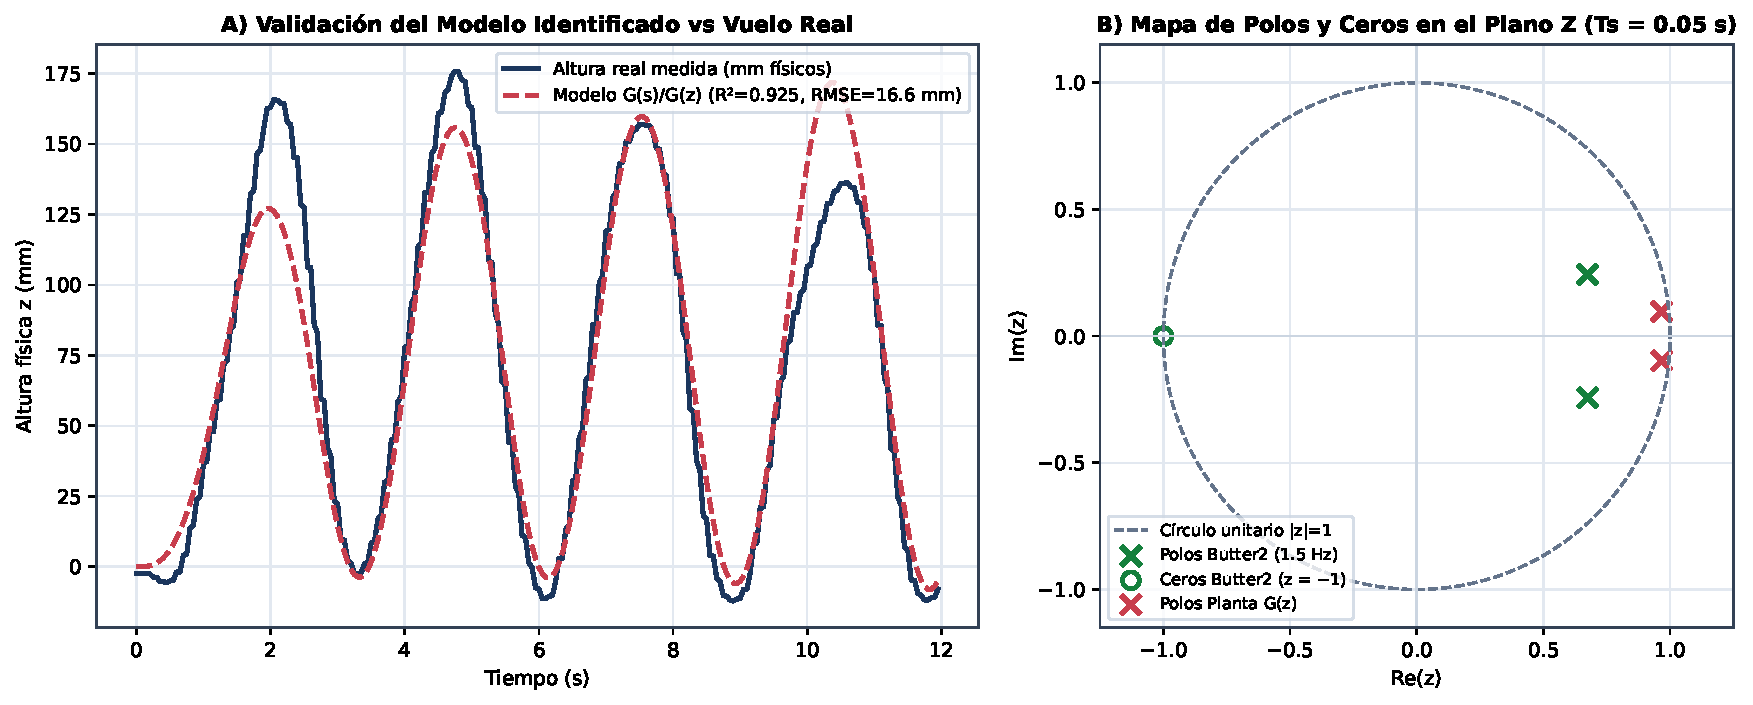
\includegraphics[width=0.95\textwidth]{fig5_identificacion_y_polos.pdf}
  \caption{A) Validaci\'{o}n del modelo continuo/discreto identificado frente a la altura f\'{i}sica real del vuelo ganador ($R^2 = 0.925$, $\text{RMSE} = 16.6\text{ mm}$). B) Mapa de polos y ceros en el plano $Z$ ($T_s = 0.05\text{ s}$) confirmando estabilidad dentro del c\'{i}rculo unitario.}
  \label{fig:ident}
\end{figure*}

\subsection{Modelo en Espacio de Estados 2-DOF}
El espacio de estados permite describir ambos grados de libertad en una sola estructura matricial \cite{cayetano_ss}. El vector de estado $\mathbf{x} = [z,\, \dot{z},\, \theta,\, \dot{\theta}]^T$ es una ``fotograf\'{i}a instant\'{a}nea'' del bic\'{o}ptero (altura, velocidad vertical, inclinaci\'{o}n y velocidad angular), impulsado por $\mathbf{u} = [\Delta u_{\text{col}},\, u_{\text{diff}}]^T$ y observado mediante $\mathbf{y} = [z,\, \theta]^T$. Con $m = 0.40\text{ kg}$, semibrazo $L = 0.075\text{ m}$ e inercia efectiva $I \approx 0.0022\text{ kg}\cdot\text{m}^2$, el modelo linealizado continuo $\dot{\mathbf{x}} = \mathbf{A}\mathbf{x} + \mathbf{B}\mathbf{u}$, $\mathbf{y} = \mathbf{C}\mathbf{x}$ resulta:
\begin{equation}
  \setlength{\arraycolsep}{2.6pt}
  \footnotesize
  \begin{aligned}
    \mathbf{A} &=
    \begin{bmatrix}
      0 & 1 & 0 & 0 \\
      -4.351 & -1.172 & 0 & 0 \\
      0 & 0 & 0 & 1 \\
      0 & 0 & 0 & -1.200
    \end{bmatrix}\!,\quad
    \mathbf{B} =
    \begin{bmatrix}
      0 & 0 \\
      20.180 & 0 \\
      0 & 0 \\
      0 & 31.533
    \end{bmatrix}\!, \\
    \mathbf{C} &=
    \begin{bmatrix}
      1 & 0 & 0 & 0 \\
      0 & 0 & 1 & 0
    \end{bmatrix}\!.
  \end{aligned}
  \label{eq:ss_cont}
\end{equation}
Su versi\'{o}n discreta ZOH a $T_s = 0.05\text{ s}$ ($\mathbf{x}[k+1] = \mathbf{\Phi}\mathbf{x}[k] + \mathbf{\Gamma}\mathbf{u}[k]$) es:
\begin{equation}
  \setlength{\arraycolsep}{2.2pt}
  \footnotesize
  \mathbf{\Phi} =
  \begin{bmatrix}
    0.9947 & 0.0485 & 0 & 0 \\
    -0.2109 & 0.9379 & 0 & 0 \\
    0 & 0 & 1.0000 & 0.0485 \\
    0 & 0 & 0 & 0.9418
  \end{bmatrix}\!,\;
  \mathbf{\Gamma} =
  \begin{bmatrix}
    0.0247 & 0 \\
    0.9782 & 0 \\
    0 & 0.0386 \\
    0 & 1.5303
  \end{bmatrix}\!.
  \label{eq:ss_disc}
\end{equation}

F\'{i}sicamente, este modelo aporta tres verificaciones directas sobre el riel:
\begin{enumerate}
  \item \textbf{Controlabilidad (rango $4/4$):} combinando empuje colectivo y diferencial es posible llevar cualquier posici\'{o}n y velocidad de altura y \'{a}ngulo al objetivo deseado.
  \item \textbf{Observabilidad (rango $4/4$):} medir \'{u}nicamente $z$ (VL53L0X) y $\theta$ (BNO055) basta para reconstruir completamente las cuatro variables internas del bic\'{o}ptero.
  \item \textbf{Eigenvalores naturales:} el eje vertical ($s = -0.586 \pm j\,2.002$; $|z| = 0.9711$) se amortigua alrededor del punto de equilibrio, mientras el eje angular posee un polo en $s = 0$ ($z = 1.0$, integrador puro): sin control retroalimentado el brazo no regresa solo a $0^\circ$, lo que explica por qu\'{e} el firmware exige siempre $K_p > 0$ en inclinaci\'{o}n.
\end{enumerate}

\section{Resultados Experimentales en Vuelo Senoidal}
La Fig.~\ref{fig:ganador} muestra la respuesta completa en el tiempo del vuelo real ganador con \texttt{Median3 + Butterworth 2\textsuperscript{o} (1.5 Hz)}. En el panel superior se aprecia c\'{o}mo la se\~{n}al filtrada elimina los picos del ToF crudo y sigue limpiamente los cuatro ciclos senoidales de $0.35\text{ Hz}$ sin golpear el tope de $1000$ u. ($\text{m\'{a}x.} = 879$ u.). En el panel central, el \'{a}ngulo relativo controlado se mantiene estable alrededor de $0^\circ$ durante todo el recorrido vertical. Finalmente, el panel inferior confirma que los dos ESCs operan de forma sim\'{e}trica y suave por encima de la base de $58\%$, sin saturaci\'{o}n destructiva ni temblor de alta frecuencia en el esfuerzo PWM ($\text{jitter} = 0.9895\%$).

\begin{figure*}[t]
  \centering
  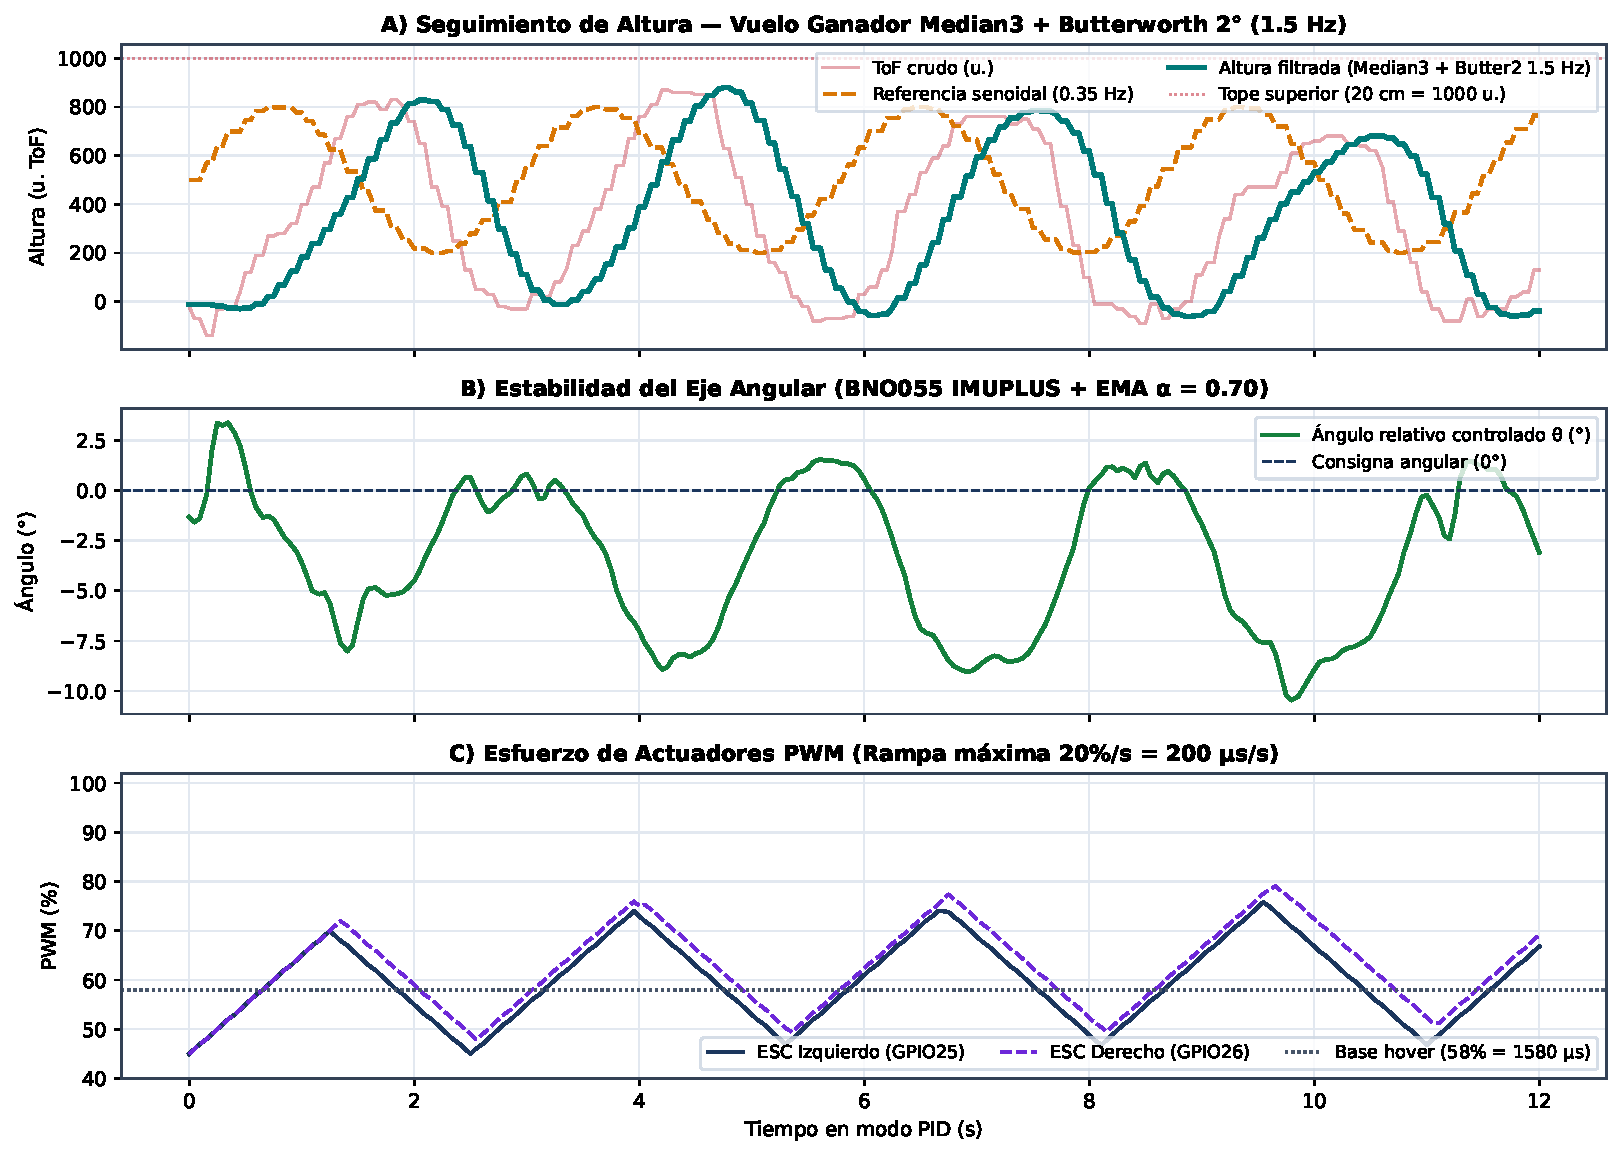
\includegraphics[width=0.95\textwidth]{fig4_vuelo_ganador_senoidal.pdf}
  \caption{Respuesta temporal completa del vuelo ganador (\texttt{Median3 + Butter2 1.5 Hz}, \texttt{COM4}, $12\text{ s}$): A) seguimiento senoidal de altura y rechazo de ruido ToF, B) estabilidad angular en $0^\circ$, y C) esfuerzo suave de los ESCs en \texttt{GPIO25/26}.}
  \label{fig:ganador}
\end{figure*}

\section{Conclusiones}
Se integr\'{o} y valid\'{o} en hardware real un sistema completo de control digital 2-DOF y filtrado DSP para un bic\'{o}ptero sobre riel vertical:
\begin{enumerate}
  \item La caracterizaci\'{o}n espectral en vuelo real demostr\'{o} que el ruido del VL53L0X es impulsivo ($33$ saltos $\ge 5\text{ mm}$ en $12\text{ s}$) y predominantemente de alta frecuencia ($59.1\%$ arriba de $2\text{ Hz}$).
  \item La combinaci\'{o}n \texttt{Median3 + Butterworth 2\textsuperscript{o} (1.5 Hz)} gan\'{o} la suite experimental de cinco filtros en vuelo real ($\text{STD} = 1.692\text{ mm}$, $\text{P2P} = 7.369\text{ mm}$, $-38.3\%$ ruido pico-a-pico frente a EMA) y qued\'{o} instalada permanentemente en el ESP32.
  \item Habilitar el cambio de filtro por puerto serial (\texttt{FILTER,0..4}) sin reiniciar el microcontrolador elimin\'{o} el problema de \textit{failsafe} en los ESCs y permiti\'{o} pruebas repetibles con observaci\'{o}n en vivo v\'{i}a SSE.
  \item El modelo experimental $G(s)/G(z)$ explic\'{o} el $92.5\%$ de la varianza del vuelo real ($R^2 = 0.9250$) y el modelo en espacio de estados confirm\'{o} controlabilidad y observabilidad totales ($4/4$), dejando lista la base para futuros controladores por realimentaci\'{o}n de estados (LQR) o sintonizaci\'{o}n fina de los cuatro reg\'{i}menes de amortiguamiento.
\end{enumerate}

\bibliographystyle{IEEEtran}
\bibliography{referencias}

\end{document}
